\chapter{ローカルデータベースに実装した読み出し試験結果検索機能の詳細と処理時間測定}

生産時には、読み出し試験の結果は一つの機関で大量に生じるものである。
4章で述べたように、任意のタイミングで必要な結果を取得できる検索機能を実装した。詳細について以下に示す。


\section{実装方法}
今回の実装では、一般的にウェブで用いられているフリーワードの検索エンジンのような機能を実装しようと考えた。
ユーザの操作を最小限にし、柔軟な検索ができるようにするためである。

また対象の読み出し試験に対しては、対象とする検索ワードを以下に絞って開発をした。
このシステムの場合、試験に関わるデータベース内の情報は固定されていて、ユーザが対象としたい検索ワードは以下の項目に限られると考えたためである。

\begin{itemize}
  \item モジュール及びFEチップのID
  \item 読み出し試験項目(例:digital scan)
  \item 読み出し試験者
  \item 読み出し試験場所
  \item 試験日時(将来的に範囲指定を用いた検索機能を検討)
  \item タグ機能を用いてつけられたタグ
\end{itemize}

そこで実装方法として、以下の2つを考えた。
\begin{enumerate}
  \item 各試験に関する情報をPythonリスト集め、検索ワードが含まれるかを確認する方法
  \item 各試験に関する情報を持つドキュメント、コレクションを予め作成、それを参照し検索を行う方法
\end{enumerate}

これらについて以下で詳細を説明する。
以下のような流れで検索処理を行う。
\begin{enumerate}
  \item ユーザが検索ワードを入力し、処理を実行
  \item 読み出し試験に関する情報を全て取得
  \item Pythonリストに保持、検索ワード一致を確認、試験を選別
  \item ブラウザーに送信
\end{enumerate}

1について、この方法のアルゴリズムのイメージを図\ref{search_python_list}に示す。
この方法はデータベース内の試験結果とアプリケーションの関数内だけで全ての処理を行うことが可能なため、シンプルな実装方法である。

\begin{figure}[bpt]
  \begin{center}
    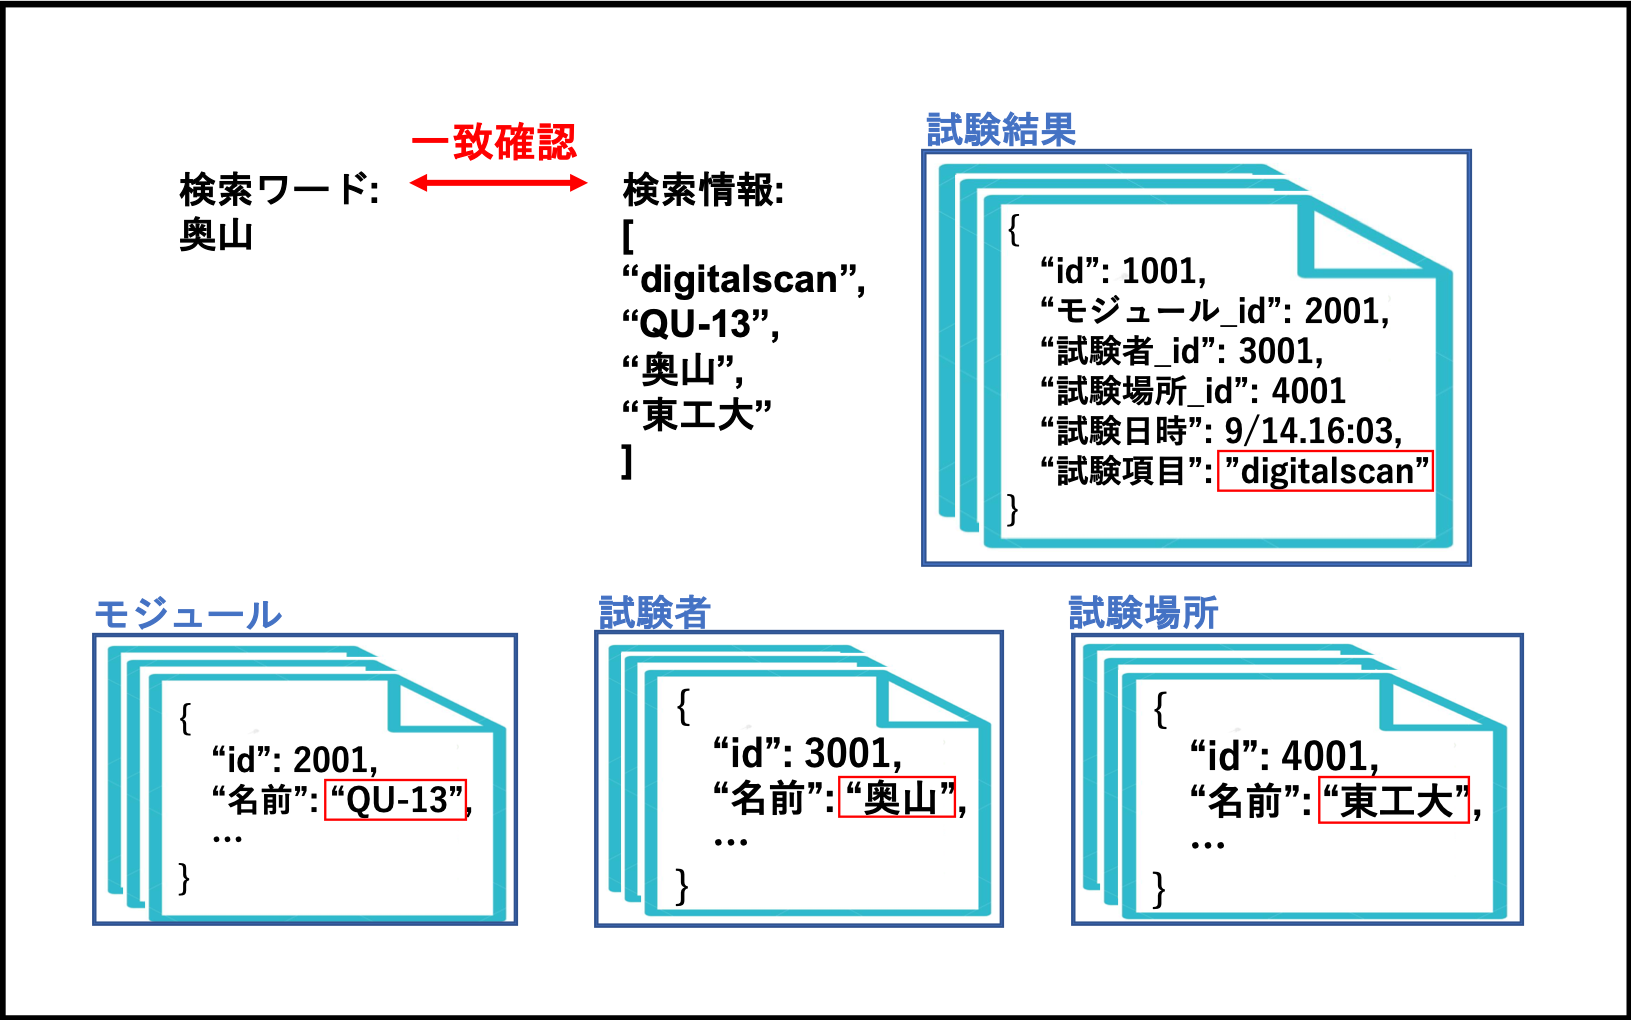
\includegraphics[width=16cm]{search_python_list}
    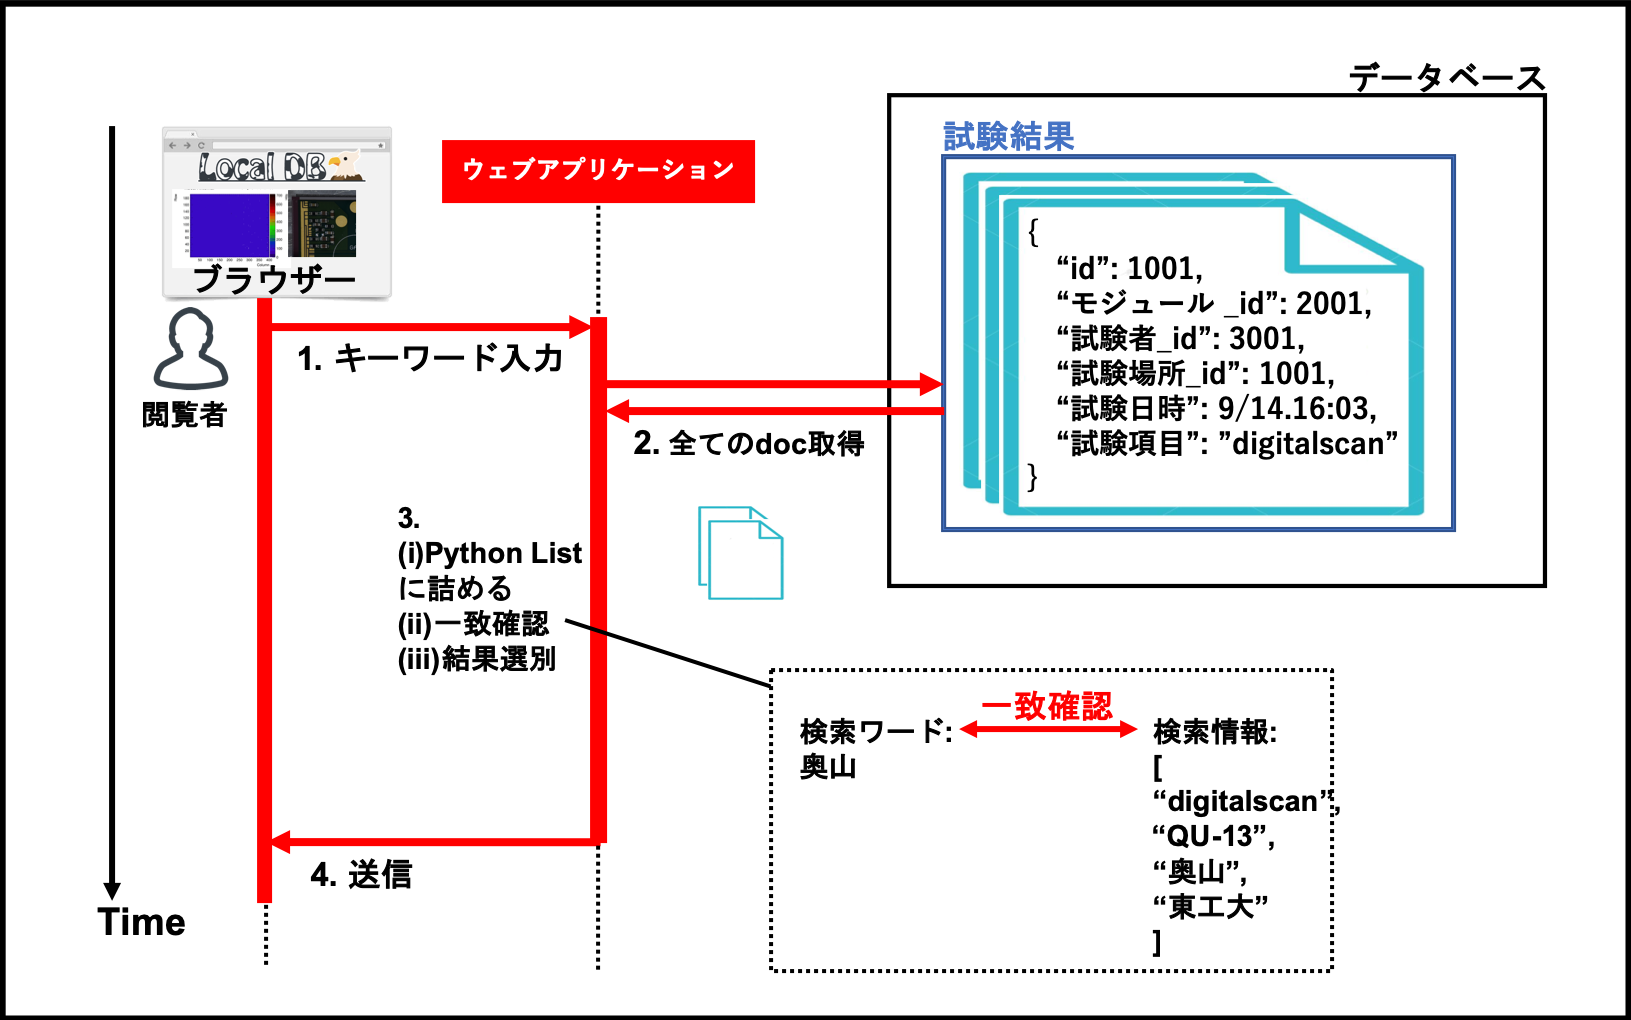
\includegraphics[width=16cm]{search_python_list_flow}
  \caption[検索機能実装方法1]{検索機能実装方法1}
  \label{search_python_list}
  \end{center}
\end{figure}


1の方法について、ユーザが処理を実行した際にデータベース内で情報を取得し、Pythonリストにつめる処理を行う。
しかしこの方法を試験実装したところ、データベース内の構造は複雑であり複数のコレクションを跨いで情報を保持しているため、試験結果全てに対してリアルタイムでこの処理を行うと、時間を大きく要してしまう問題が発生した。
イメージを図\ref{search_python_list_problem}に示す。

そこで方法2を考案し、実装を行った。アルゴリズムのイメージを図\ref{search_mongo_collection}に示す。
検索キーワードを別のドキュメントに予め保持しておき、処理実行時にはそれを参照することで検索を行うというものである。


\section{処理時間測定}
 
\section{いくつかの改善点と比較}

